\documentclass[letterpaper,12pt]{scrartcl}
\usepackage{epsfig,latexsym,amsmath,amssymb,epic,eepic,psfrag,subfigure,float,euscript,array}
\usepackage[latin1]{inputenc}
\usepackage[margin=24mm]{geometry}
\usepackage{enumitem}
\usepackage{tikz,pgf,pgfplots}
\usepgfplotslibrary{fillbetween}
\usetikzlibrary{decorations, arrows, patterns}

\usepackage[absolute]{textpos}
\usepackage{adjustbox}
\usepackage[amssymb]{SIunits}

\usepackage{array}
\newcolumntype{L}{>{\[}l<{\]}} % math-mode version of "l" column type

\newenvironment{exercise}[1][Problem]{\begin{trivlist} \item[\hskip
    \labelsep {\stepcounter{exerctr}\bfseries #1
      \arabic{exerctr}}]}{\end{trivlist}\vspace{10mm}}

\newcounter{exerctr}
\newcounter{abcctr}[exerctr]

\newcommand{\abc}{\noindent\vspace{1mm}\\ {\bf
    \stepcounter{abcctr}(\alph{abcctr})\ }}
\newcommand{\bbm}{\begin{bmatrix}}
\newcommand{\ebm}{\end{bmatrix}}
\newcommand{\point}[1]{\hfill {\bf (#1p)}\\ \vspace{-5mm}}
\newcommand{\ctrb}{\EuScript{S}}
\newcommand{\Lap}{\mathcal{L}}
\newcommand{\obsv}{\EuScript{O}}
\newcommand{\realdel}{\text{Re}}
\newcommand{\imagdel}{\text{Im}}
\newcommand{\bC}{\mathbb{C}}
\newcommand{\bR}{\mathbb{R}}
\newcommand{\bmpv}{\begin{minipage}[t]}
\newcommand{\bmps}{\begin{minipage}[t]{45mm}}
\newcommand{\bmpm}{\begin{minipage}[t]{90mm}}
\newcommand{\bmpl}{\begin{minipage}[t]{\textwidth}}
\newcommand{\emp}{\end{minipage}}
\newcommand{\mexp}[1]{\ensuremath{\mathrm{e}^{#1}}}
\newcommand*{\laplaceinv}[1]{\ensuremath{\mathcal{L}^{-1} \left\{#1\right\}}}
\newcommand*{\ztrf}[1]{\ensuremath{\mathcal{Z} \left\{#1\right\}}}
\newcommand*{\shift}{\ensuremath{\operatorname{q}}}
\newcommand*{\diff}{\ensuremath{\operatorname{p}}}

\newcommand\tikzmark[2]{\tikz[overlay, remember picture, anchor=base] \node (#1) {#2};}
\newcommand\tikzmathmark[2]{\tikz[remember picture, inner sep=0pt, outer sep=0pt, baseline, anchor=base] \node (#1) {\ensuremath{#2}};}


\addtolength{\topmargin}{-8mm}
%\textheight 22.5cm
%\oddsidemargin 1.3cm
%\evensidemargin 1.3cm

\makeatletter
\newcommand*{\rom}[1]{\expandafter\@slowromancap\romannumeral #1@}
\makeatother

\newcommand*\circled[1]{\tikz[baseline=(char.base)]{
            \node[shape=circle,draw,inner sep=2pt] (char) {#1};}}


\title{Computerized Control Final exam (28\%)}
\author{Kjartan Halvorsen}
%\date{}

\begin{document}

\begin{textblock}{13}(1,0.6)
\fbox{
\bmpl%
{\bf Matricula and name:}\\
\vspace*{4mm}
\emp}
%\noindent\large\bf Matricula and name:
\end{textblock}


{\let\newpage\relax\maketitle}


\begin{description}
\item[Time] Thursday November 28 19:10 --- 21.55
\item[Place] 5305
\item[Permitted aids] The single colored page with your own notes, table of Laplace transforms, calculator
\end{description}

All answers should be readable and well motivated (if nothing else is written). Solutions/motivations should be written on the provided spaces in this exam. 

\begin{center}
{\Large Good luck!} \\
\end{center}


\clearpage

%-----------------------------------------------------------------
% Exercise 1. State-space 
%-----------------------------------------------------------------
\begin{exercise}

The linearized inverted-pendulum model is used in the control design for many types of systems, such as rockets and segways. 
\begin{center}
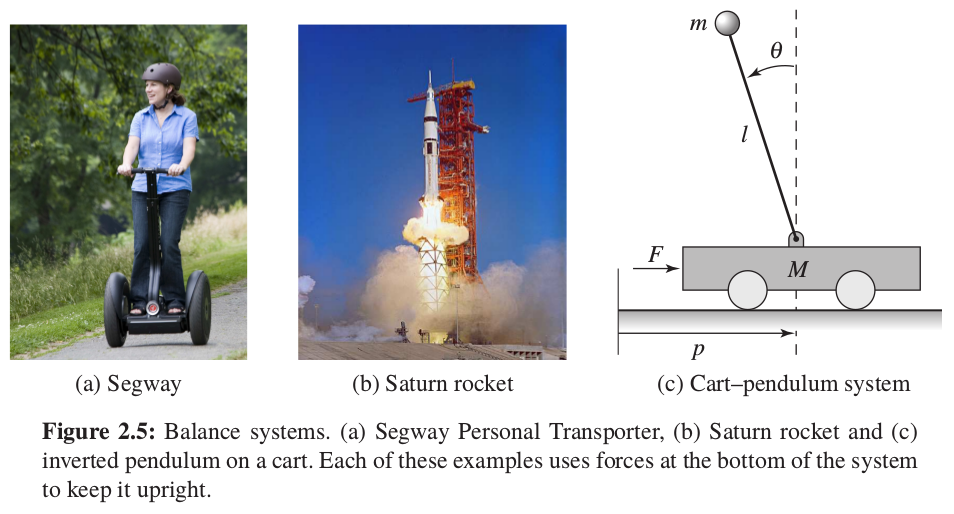
\includegraphics[width=0.7\linewidth]{AM_fig2_5.png}\\
{\small From \AA{}str\"om \& Murray ``Feedback systems'' Princeton University Press, 2008.}
\end{center}
In the continuous-time domain the system has the transfer function 
\begin{equation}
G(s) = \frac{\omega_0^2}{s^2 - \omega_0^2}.
\label{eq:ctmodel}
\end{equation}
It can also be described in discrete-time as the state-space model
\begin{equation}
  \begin{aligned}
    x(k+1) &= \underbrace{\bbm 2\cosh(\omega_0h) & 1\\-1 & 0\ebm}_{\Phi} x(k) + \underbrace{\bbm \cosh(\omega_0h)-1\\\cosh(\omega_0h)-1\ebm}_{\Gamma} u(k)\\
    y(k) &= \underbrace{\bbm 1 & 0 \ebm}_{C} x(k)
  \end{aligned}
\label{eq:dtmodel}
\end{equation}
 Note that $\cosh(\omega_0h) = \frac{1}{2}( \mexp{\omega_0 h} + \mexp{-\omega_0 h})$.

\abc
Assume that we want to control the inverted pendulum using linear state feedback so that the closed-loop system  has a step-response as shown in figure \ref{fig:stepresponse}. Determine a suitable sampling period $h$ for the system, in terms of $\omega_0$.

\noindent
\fbox{
\bmpl
{\bf Answer and motivation for sampling period $h$:}\\
\vspace*{30mm}
\emp}
\begin{figure}
  \begin{center}
    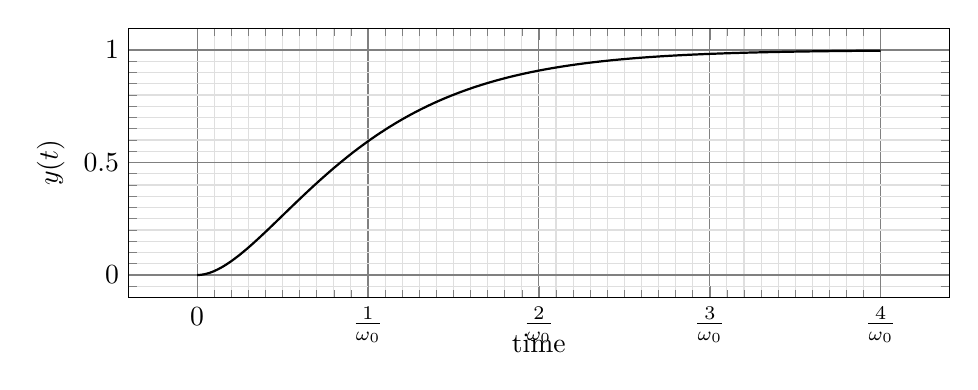
\begin{tikzpicture}
      
      \pgfmathsetmacro{\wnoll}{2}
      \begin{axis} [
        width=12cm,
        height=5cm,
        xlabel = {time},
        ylabel = {$y(t)$},
        xtick = {0,1,2,3,4},
        xticklabels={0, $\frac{1}{\omega_0}$, $\frac{2}{\omega_0}$, $\frac{3}{\omega_0}$, $\frac{4}{\omega_0}$},
        x label style={at={(axis description cs:0.5,-0.1)},anchor=north},
        grid = both,
        minor tick num=9,
        minor grid style={gray!25},
        major grid style={black!50},
        ]
         \addplot+[thick, black, solid, no marks, domain=0:4, samples=400] { 1  - exp(-\wnoll*x) - \wnoll*x*exp(-\wnoll*x)};
      \end{axis}
    \end{tikzpicture}
    \caption{Step-response of desired closed-loop system (in continuous-time)}
    \label{fig:stepresponse}
  \end{center}
\end{figure}

\abc
Determine the \textbf{poles} of the continuous-time system \eqref{eq:ctmodel} and the discrete-time model \eqref{eq:dtmodel}, making use of the sampling period $h$ you decided in (a). Also,  \textbf{mark} the poles in figure \ref{fig:planes}.
\begin{figure}[h]
\begin{center}
  \begin{tikzpicture}
    \def\alength{3}
    \draw[->] (-\alength,0) to (\alength,0) node[below] {Re};
    \draw[->] (0, -\alength,0) -- node[left,pos=0.95] {Im} (0, \alength,0) ;
    \node[anchor=south] at (0,\alength) {s-plane};

    \begin{scope}[xshift=9cm]
      \draw[->] (-\alength,0) to (\alength,0) node[below] {Re};
      \draw[->] (0, -\alength,0) -- node[left,pos=0.95] {Im} (0, \alength,0) ;
      \node[anchor=south] at (0,\alength) {z-plane};
      \node[circle, draw, minimum width=4cm] at (0,0) {};
      \node[coordinate, pin=-45:{1}] at (2,0) {};
    \end{scope}
    
  \end{tikzpicture}
  \caption{Mark the poles of the continuous-time system \eqref{eq:ctmodel} and the discrete-time system \eqref{eq:dtmodel}.}
  \label{fig:planes}
\end{center}
\end{figure}
\noindent
\fbox{
\bmpl
{\bf Calculation of continuous- and discrete poles:}\\
\vspace*{60mm}
\emp}

\abc
Is the discrete-time state-space model~\eqref{eq:dtmodel} \textbf{observable}?

\noindent
\fbox{
\bmpl
{\bf Calculations:}\\
\vspace*{90mm}
\emp}

\abc for a specific choice of sampling period $h$ we obtain the following discrete-time state-space model for the linearized inverted pendulum
\begin{equation}
  \begin{aligned}
    x(k+1) &= \bbm 2.04 & 1\\-1 & 0\ebm x(k) + \bbm 0.02\\0.02 \ebm u(k)\\
    y(k) &= \bbm 1 & 0 \ebm x(k)
  \end{aligned}
\label{eq:dtmodelnum}
\end{equation}
The following control law has been designed \[u(k) = -Lx(k) + l_0y_{ref}(k) = -19x_1(k) - 15x_2(k) + 2.7y_{ref}(k),\] which gives a closed-loop system with step-response close to the desired response in figure \ref{fig:stepresponse}. However, only measurements of the output $y(k)$ of the system are available, so it is necessary to use an observer. 
Which of the following state-space expressions is the correct one for the observer? No motivation required.
\begin{enumerate}
\item \( \hat{x}(k+1) = \Phi \hat{x}(k) + \Gamma u(k) \)
\item \( \hat{x}(k+1) = \Phi \hat{x}(k) + \Gamma u(k) + K(y(k) -\hat{x}(k)) \)
\item \( \hat{x}(k+1) = \Phi \hat{x}(k) + \Gamma u(k) - K\hat{x}(k) \)
\item \( \hat{x}(k+1) = \Phi \hat{x}(k) + \Gamma u(k) + Ky(k) -KC\hat{x}(k) \)
\end{enumerate}

\abc
With the state-space model~\eqref{eq:dtmodelnum}, determine an observer gain vector such that the observer has all its poles in the origin (deadbeat observer).

\noindent
\fbox{
\bmpl
{\bf Calculations:}\\
\vspace*{130mm}
\emp}

\abc
The output feedback controller when it is designed (gain vectors $L$ and $K$ determined) corresponds to a discrete-time dynamical system with two input signals and one output signal. The input signals are  the reference signal $y_{ref}(k)$ and the feedback signal $y(k)$, and the output signal is the control signal $u(k)$. 
\begin{center}
  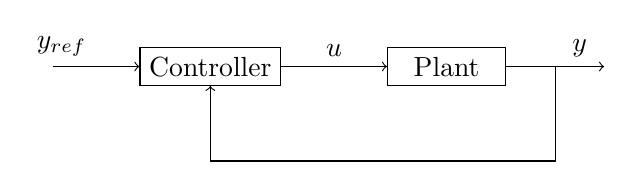
\begin{tikzpicture}[node distance=22mm, block/.style={rectangle, draw, minimum width=15mm}, sumnode/.style={circle, draw, inner sep=2pt}]
    
    \node[coordinate] (input) {};
    \node[block, right of=input, node distance=20mm] (controller)  {Controller};
    \node[block, right of=controller, node distance=30mm] (plant)  {Plant};
    \node[coordinate, right of=plant, node distance=20mm] (output) {};

    \draw[->] (input) -- node[above, pos=0.1] {$y_{ref}$} (controller);
    \draw[->] (controller) -- node[above, pos=0.5] {$u$} (plant);
    \draw[->] (plant) -- node[above, near end] {$y$} node[coordinate] (measure) {} (output);
    \draw[->] (measure) -- ++(0,-12mm) -| (controller);
  \end{tikzpicture}
\end{center}

On state space form this controller corresponds to the system
\begin{equation}
  \begin{aligned}
    \hat{x}(k+1) &= \left( \Phi - \Gamma L - KC \right) \hat{x}(k) + l_0\Gamma y_{ref}(k) + Ky(k)\\
    u(k) &= -L\hat{x}(k) + l_0y_{ref}(k)
  \end{aligned}
\label{eq:observer}
\end{equation}
 This system can of course also be written on transfer-function form. For the particular system in this exercise, the controller becomes
\begin{equation}
  u(k) = F_f(\shift)y_{ref}(k) - F_b(\shift)y(k) = \frac{2.7\shift^2 + 1.8\shift + 0.8}{\shift^2 + 1.365\shift + 0.68}y_{ref}(k) - \frac{24.2\shift - 11.1}{\shift^2 + 1.365\shift + 0.68}y(k).
  \label{eq:controller}
\end{equation}
Write the controller as a \textbf{difference equation} with the newest value of $u$ by it self on the left-hand side, just as you would write it in order to implement the controller in code (for instance on an arduino).

\noindent
\fbox{
\bmpl
{\bf Calculations:}\\
\vspace*{110mm}
\emp}


\end{exercise}

% -----------------------------------------------------------------
% Exercise 2. Match pulse-transfer function with step-response
%-----------------------------------------------------------------
\begin{exercise}

For each of the four pulse-transfer functions below, determine which of the step-responses in figure \ref{fig:steps} it corresponds to.
\begin{align*}
  G_1(z) &= \frac{0.02(z + 0.95)}{(z-0.8)(z-1.2)}\\
  G_2(z) &= \frac{0.08(z + 0.95)}{(z-0.6)^2}\\
  G_3(z) &= \frac{0.02(z + 0.95)}{(z-0.8+0.5i)(z-0.8-0.5j)}\\
  G_4(z) &= \frac{z + 0.95}{(z-1)(z-0.8)}\\
\end{align*}

\begin{figure}[hbtp]
\begin{center}
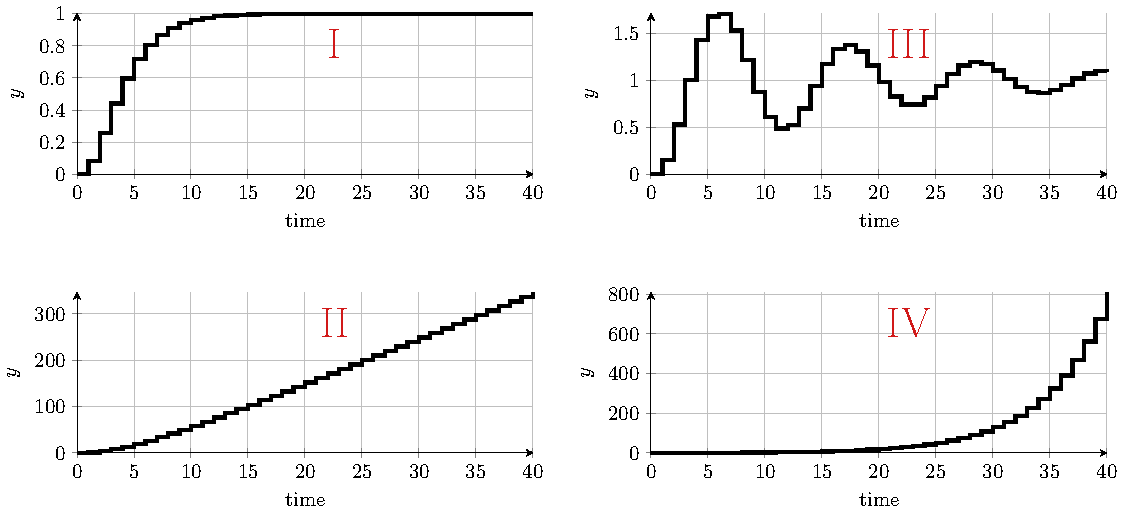
\includegraphics[width=\linewidth]{step-responses-fall19}
\caption{Exercise \arabic{exerctr} Match the step-responses with the pulse-transfer functions.}\label{fig:steps}
\end{center}
\end{figure}

\noindent
\fbox{
\bmpl%
{\bf Answer and motivation:}\\
\vspace*{110mm}
\emp}

\end{exercise}

%\cleardoublepage%
%\end{document}


\section*{Solutions}

\setcounter{exerctr}{0} 

\begin{exercise}
\abc%
Choosing a suitable sampling period is based on the speed of either the open-loop system or the desired closed-loop system. Here we are given a desired step-response of the closed-loop system. One common rule-of-thumb is that we should have 4 to 10 samples in one rise-time. The rise-time is from 10\% to 90\% of the final value which gives (approximately) $t_r = \frac{2}{\omega_0} - \frac{0.3}{\omega_0} = \frac{1.7}{\omega_0}$. Since the open-loop system is unstable, it is good to be cautious and choose a short sampling period, for instance
\[ h = \frac{0.2}{\omega_0}.\]
\abc%
For the continuous-time system the characteristic equation is 
\( s^2 - \omega_0^2 = 0\) with solutions \[s = \pm \omega_0.\]
For the discrete-time state-space system the poles are the eigenvalues of the $\Phi$-matrix. The characteristic equation becomes
\begin{equation*}
  \begin{aligned}
    \det \left( zI - \Phi\right) &= 0\\
    \det \bbm z - 2\cosh(\omega_0h) & -1\\1 & z \ebm &= 0\\
    (z-2\cosh(\omega_0h))z + 1 &= 0\\
    z^2 - 2\cosh(\omega_0h)z + 1 &= 0\\
    z^2 - \big(\mexp{\omega_0h} + \mexp{-\omega_0h}\big)z + 1 &= 0\\
    \big(z - \mexp{\omega_0h0}\big)\big(z - \mexp{-\omega_0h}\big) &= 0.
  \end{aligned}
\end{equation*}
With solutions 
\[z_1 = \mexp{\omega_0h} = \mexp{0.2} \approx 1.22,\qquad  z_1 = \mexp{-\omega_0h} = \mexp{-0.2} \approx 0.82.\]
\begin{center}
  \begin{tikzpicture}
    \def\alength{3}
    \draw[->] (-\alength,0) to (\alength,0) node[below] {Re};
    \draw[->] (0, -\alength,0) -- node[left,pos=0.95] {Im} (0, \alength,0) ;
    \node[anchor=south] at (0,\alength) {s-plane};
    \node[pin=-90:{$-\omega_0$}] at (-2,0) {\large $\times$};
    \node[pin=-90:{$\omega_0$}] at (2,0) {\large $\times$};
    \begin{scope}[xshift=9cm]
      \draw[->] (-\alength,0) to (\alength,0) node[below] {Re};
      \draw[->] (0, -\alength,0) -- node[left,pos=0.95] {Im} (0, \alength,0) ;
      \node[anchor=south] at (0,\alength) {z-plane};
      \node[circle, draw, minimum width=4cm] at (0,0) {};
      \node[pin=-120:{$\mexp{-\omega_0h}$}] at (1.7,0) {\large $\times$};
      \node[pin=-60:{$\mexp{\omega_0h}$}] at (2.3,0) {\large $\times$};
    \end{scope}
    
  \end{tikzpicture}
\end{center}

\abc%
To check for observability, form the observability matrix which for a second-order system is 
\[W_o = \bbm C\\C\Phi \ebm,\]
and check that it is non-singular (that its determinant is not zero). We get
\[W_o = \bbm C\\C\Phi \ebm = \bbm 1 & 0\\2\cosh(\omega_0 h) & 1\ebm, \]
with determinant
\[ \det W_o = 1 \neq 0, \]
so the system is \textbf{observable}. In fact, the system is on observable canonical form, which means it must be observable. 

\abc%
The correct expression for the observer is 
\[ hat{x}(k+1) = \Phi \hat{x}(k) + \Gamma u(k) + Ky(k) -KC\hat{x}(k). \]

\abc%
The poles of the observer are given by the solutions to the characteristic equation
\[ \det \big(zI -  (\Phi - KC)\big) = 0.\]
Since $K=\bbm k_1 & k_2 \ebm^T$, 
\[ KC = \bbm k_1 & 0\\k_2 & 0\ebm\]
and 
\[ \Phi - KC = \bbm 2\cos(\omega_0 h) - k_1 & 1\\-1-k_2 & 0\ebm \]
the characteristic polynomial becomes 
\[ \det  \big(zI -  (\Phi - KC)\big) = \det \bbm z-2\cosh(\omega_0h)+k_1 & -1\\1+k_2 & z \ebm = z^2 + \big(k_1-2\cosh(\omega_0 h)\big)z + 1+k_2.\]
Compare this with the desired characteristic polynomial for a deadbeat observer, which is $z^2$, to get the following equations for the observer gains
\begin{align*}
  k_1 - 2\cosh(\omega_0 h) &=0\\
  1+k_2 &= 0
\end{align*}
with the obvious solution
\[ k_1 = 2\cosh(\omega_0h) = 2.04, \qquad k_2 = -1. \] 

\abc%
The difference equation becomes
\[ (\shift^2 + 1.365\shift + 0.68)u(k) = (2.7\shift^2 + 1.8\shift + 0.8)y_{ref}(k) - (24.2\shift -11.1)y(k)\]
\[  u(k+2) + 1.365u(k+1) + 0.68u(k) = 2.7y_{ref}(k+2) + 1.8y_{ref}(k+1) + 0.8y_{ref}(k) - 24.2y(k+1) + 11.1y(k)\]
Shifting the difference equation back in time with two sampling period (multiplying both sides with $\shift^{-2}$) and rearranging gives 
\[ u(k) = -1.365u(k-1) - 0.68u(k-2) + 2.7y_{ref}(k) + 1.8y_{ref}(k-1) + 0.8y_{ref}(k-2) - 24.2y(k-1) + 11.1y(k-2). \]
This is what is implemented in the computer. 
\end{exercise}


\begin{exercise}
\pgfmathsetmacro{\omegan}{sqrt(1+pow(0.6, 2))}
\pgfmathsetmacro{\omeganhertz}{\omegan * 1000/2/pi}
\pgfmathsetmacro{\hh}{0.2}
\pgfmathsetmacro{\pdreal}{exp(-\hh)*cos(deg(0.6*\hh))}
\pgfmathsetmacro{\pdim}{exp(-\hh)*sin(deg(0.6*\hh))}

The idea is to figure out the poles of the four systems, and from this determine how the system should respond.

The system $G_1(z)$ poles in $z=0.8$ and $z=1.2$, the latter of which is outside the unit circle. This gives a diverging response. The system $G_2(z)$ is critically damped with two poles in $z=0.6$. This has a stable, fast response with no overshoot. System $G_3(z)$ has complex-conjugated poles in $z = 0.8 \pm i0.5$ which are inside the unit circle, but with poor damping. This gives an oscillating, stable response. Finally, $G_4(z)$ has poles in $z=1$ and $z=0.8$, and so it contains an integration, and the response will grow with time. The analysis leads to the pairing: \textbf{$G_1(z)$ --- \rom{4}},  \textbf{$G_2(z)$ --- \rom{1}},  \textbf{$G_3(z)$ --- \rom{3}},  \textbf{$G_4(z)$ --- \rom{2}}. 
\end{exercise}
\end{document}
